\documentclass[11pt]{article}
\usepackage[margin=1in]{geometry}
\usepackage[T1]{fontenc}
\usepackage[utf8]{inputenc}
\usepackage{mathptmx}
\usepackage{microtype}
\usepackage{amsmath}
\usepackage{booktabs}
\usepackage{multirow}
\usepackage{graphicx}
\usepackage{caption}
\usepackage{xcolor}
\usepackage[numbers,sort&compress]{natbib}
\usepackage[hidelinks]{hyperref}
\captionsetup{font=small,labelfont=bf,skip=6pt}
\setlength{\parskip}{3pt}
\newcommand{\pz}{P\textsubscript{0}}
\newcommand{\po}{P\textsubscript{1}}
\newcommand{\pt}{P\textsubscript{2}}
\newcommand{\dAUROC}{\ensuremath{\Delta\mathrm{AUROC}}}

\title{\textbf{Minimum Evidence, Maximum Utility?}\\[4pt]
\large Measuring Data-Minimization Cost and Evidence-Acquisition Value for Tabular AI Across Four Domains}
\author{Michael P.\ Ryder, DO\\ \small Independent researcher \\ \small \texttt{michaelryder.do@gmail.com}}
\date{\small Preprint --- September 2026. Pre-registered designs; every number is read from committed, content-addressed result files.}

\begin{document}
\maketitle

\begin{abstract}
\noindent Two questions sit on the same axis of a tabular analysis. \emph{Minimization}: how much of the available evidence can be removed before predictive utility changes, and is the answer the same for every model? \emph{Acquisition}: given what is already known about a case, which missing category of evidence would most change the current inference? We address both with a shared, fixed evaluation environment, three producers (logistic regression, histogram gradient boosting, and a frozen tabular foundation-model probe), and pre-registered verdict rules. \textbf{Study 1} places four public or synthetic tasks---clinical utilization, industrial machine failure, consumer purchase intent, and regulatory permit status---on a three-rung evidence ladder and measures split-replicated paired \dAUROC{} with 95\% $t$-intervals ($K=20$ or $10$ grouped splits). The minimization frontier is producer- and task-dependent: on the clinical task the governed step improved logistic regression ($+0.024$ [$+0.006$, $+0.042$]), cost the tree model ($-0.028$ [$-0.047$, $-0.010$]) and left the probe unchanged ($+0.005$ [$-0.010$, $+0.020$]); on the regulatory task, whose ladder coarsens location rather than removing fields, the same governed step cost the probe ($-0.016$ [$-0.027$, $-0.006$]) and the tree model but not logistic regression. Aggressive minimization cost eleven of twelve producer--task cells, from $-0.013$ to $-0.162$; the twelfth (clinical logistic regression, $-0.022$ [$-0.044$, $+0.000$]) was recorded as no measured cost because its interval reached zero. The probe had the highest replicated mean at ten of eleven task--level cells, and at the clinical governed level it reversed a single-split comparison that had placed logistic regression ahead. \textbf{Study 2} evaluates whether the frozen probe can rank withheld evidence classes by the change in its own inference that revealing them produces, validating by reveal rather than by attention scores. Across 20 clinical splits, ranking accuracy was $0.797$ [$0.780$, $0.813$] with every split clearing a pre-set usefulness bar; the single pre-registered split had given $0.874$. Accuracy rose with the number of donor imputations ($0.789$--$0.906$) and on two further tasks was $0.821$ (46\% of cases excluded as indistinguishable) and $0.915$/$0.900$ (11--13\% excluded). Both studies were corrected by their own replications, and both corrections are reported. A pre-registered replication in miniature on 242 origin rows from 100 real de-identified patients (MIMIC-IV demo) reproduced the producer-dependence of the governed step and the acquisition result ($0.828$ [$0.802$, $0.854$]) but not the uniform aggressive cost: on that cohort the aggressive step improved the linear model. The claims are bounded: no formal privacy guarantee, no causal importance, no decision rule, and no generalisation beyond the tested tasks, producers and ladders.
\end{abstract}

\section{Introduction}

Data minimization is a legal principle~\citep{gdpr} and an engineering habit, but its cost to a predictive model is usually asserted rather than measured. One assertion is that a well-chosen minimization is free; the opposite is that every field removed costs a fixed increment of accuracy. Neither is a measurement. The complementary question---which \emph{missing} evidence would most change a model's current inference---is the classical value-of-information problem~\citep{howard1966} in the language of active feature acquisition~\citep{saartsechansky2009,shim2018}, and in practice it is often answered by reading a model's attention or feature-importance scores as if they were validated measurements. They are internal signals.

This paper treats both questions as measurements with pre-registered designs and reports what the measurements showed, including two places where a replication corrected the first result. The two studies share one evaluation environment, one probe, and one discipline: hypotheses and verdict rules were fixed before the runs, every result file is content-addressed and committed, and the public phrasing of each finding was written against an explicit claims boundary that names what the evidence does \emph{not} support.

Our contributions are empirical. (i)~Across four tasks with materially different data---synthetic clinical records, machine telemetry, web-session behaviour, and geospatial regulatory records---the cost of minimization is a measured curve with intervals, per producer and per task, not a constant (Section~\ref{sec:study1}). (ii)~The same governed minimization step can improve one producer while costing another on the same task, and can be free on one task's axis while costly on another's. (iii)~A frozen tabular foundation model can rank withheld evidence classes by the change revealing them actually produces, well above chance and above a pre-set usefulness bar, on three tasks; the size of that number depends on protocol parameters that we report alongside it (Section~\ref{sec:study2}). (iv)~In both studies the first, single-split result was materially revised by split replication, in one case reversing a model ranking; we argue that the correction trail is part of the method (Section~\ref{sec:discussion}).

\section{Shared evaluation environment}
\label{sec:env}

All analyses were run in a fixed provenance-preserving evaluation environment that held representations, splits, and producer identity constant across evidence levels. Concretely: each evidence level is a \emph{projection} of the source table whose definition and content are content-addressed (SHA-256); producers see only the projected fields for their level; the projection hash, the split identity, and the producer identity are recorded with every cell; and a harness code digest is written into every report. No result in this paper was re-estimated for the write-up.

\paragraph{Producers.} Logistic regression (standardised features, $L_2$, fixed seed), histogram gradient boosting (HistGB, fixed seed)~\citep{sklearn}, and a frozen tabular foundation-model probe: TabICL~v2~\citep{tabicl}, BSD-3-Clause, checkpoint pinned by SHA-256 (\texttt{bdc7dbd5\ldots}, 110{,}368{,}038 bytes) and verified before each run. The probe is used as an instrument---a fixed function from a projected table to held-out probabilities---not as the object of study. Trivial and heuristic producers exist in the harness and are not part of the frontier result.

\paragraph{Splits and statistics.} Splits are grouped hash splits: a unit (patient, machine, session, facility) is assigned to the test fold when $\mathrm{sha256}(\text{split\_id}\!:\!\text{group\_id})$ falls in the lower 30\% of its range. Replicates change the split identity only; producer seeds are fixed, so the replicated factor is the split. The outcome is AUROC on held-out units. Study~1 reports paired per-split \dAUROC{} between adjacent evidence levels with mean, standard deviation and a 95\% Student-$t$ interval over the $K$ splits. The verdict rule was fixed before any run: an interval entirely above zero is \emph{improves}, one covering zero is \emph{no measured cost}, one entirely below zero is \emph{costs utility}.

\paragraph{Evidence ladders.} Three rungs per task. \pz{} is the maximum permissible feature set for the task (fields that would leak the label window are excluded at every rung). \po{} is a \emph{governed} projection: only fields that survive a fixed governed projection, with features derived solely from surviving fields. \pt{} is aggressive minimization: a named handful of \po-derivable aggregates. Which fields each rung contains is recorded by hash; code vocabularies are chosen by prevalence only, never by association with the target.

\paragraph{Pre-registration and the claims boundary.} Each study's design, metrics, and verdict rules were written before its runs, with amendments recorded in the plan file rather than applied silently. Alongside the plans we maintained a claims boundary: a list of sentences the evidence supports and a list it does not. Every statement below was checked against it.

\section{Study 1: Data minimization across four domains}
\label{sec:study1}

\subsection{Design}

\begin{table}[t]
\centering\small
\caption{Tasks in the minimization study. $K$ is the number of grouped split replicates. Fields per rung are the projection widths after one-hot encoding.}
\label{tab:tasks}
\begin{tabular}{@{}p{3.6cm}p{5.2cm}rrp{2.1cm}p{2.0cm}@{}}
\toprule
Task & Source (licence) & $n$ & $K$ & \pz/\po/\pt{} fields & Minimization axis \\
\midrule
Healthcare: acute utilization within 365 d & Synthea synthetic records~\citep{synthea}; 111 patients $\to$ 1{,}044 rolling-origin rows & 1{,}044 & 20 & 96 / 83 / 10 & field removal \\
Manufacturing: machine failure & AI4I 2020~\citep{ai4i} (CC BY 4.0) & 10{,}000 & 10 & 9 / $\equiv$\pz{} / 3 & field removal \\
Consumer: purchase intent & UCI Online Shoppers~\citep{shoppers} (CC BY 4.0) & 12{,}330 & 10 & 56 / 24 / 5 & field removal \\
Regulatory: facility absent from permit records & Cal-FF~\citep{calff} (CC0-1.0); 2{,}121 facilities & 2{,}121 & 10 & 23 / 19 / 6 & location precision \\
\bottomrule
\end{tabular}
\end{table}

Table~\ref{tab:tasks} lists the four tasks. Three place fields on the ladder by removal. The manufacturing task has no distinct \po{}: its governed projection retains all nine fields, so only \pt$-$\pz{} is tested there. The consumer \po{} drops device and network context codes; \pt{} keeps five behavioural fields. The regulatory task places \emph{location precision} on the ladder instead: \pz{} carries exact coordinates and bounding box, \po{} carries county membership only, \pt{} carries structural and animal-type fields with no location. Its label---no state permit within 1{,}000~m of the facility centroid, 265 positives, base rate $0.125$---is a pre-registered construction that is not the source paper's matcher (which reports 222 unpermitted facilities); alternative radii were recorded (500~m: 485; 2{,}000~m: 113) and never used for tuning. A fifth candidate domain (a governance-log regression target) was assessed first and excluded as inadequate for the design; it is not reported.

\subsection{Results}

\begin{figure}[t]
\centering
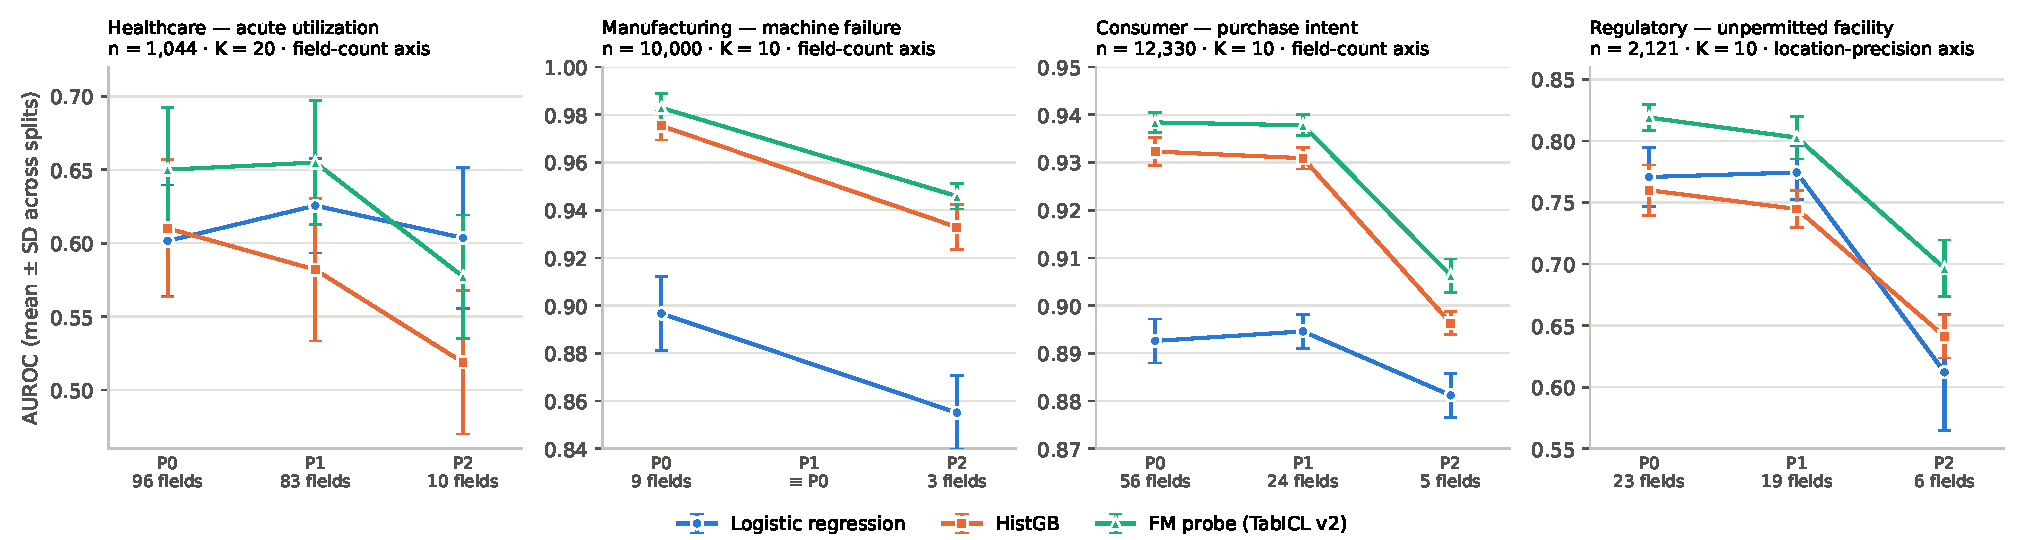
\includegraphics[width=\textwidth]{figs/fig1_frontier_4dom.pdf}
\caption{Utility versus evidence level for three producers on four tasks. Points are mean AUROC over $K$ grouped splits; whiskers are $\pm 1$~SD across splits and are descriptive. Inference is carried by the paired per-split deltas in Figure~\ref{fig:forest}. Note the healthcare panel, where the three producers respond differently to the same governed step, and the regulatory panel, where the governed step coarsens location.}
\label{fig:frontier}
\end{figure}

\begin{table}[t]
\centering\small
\caption{Replicated AUROC by evidence level: mean (SD) over $K$ grouped splits. The probe has the highest mean at ten of the eleven task--level cells; the exception is clinical \pt{}, where logistic regression is ahead.}
\label{tab:means}
\begin{tabular}{@{}llccc@{}}
\toprule
Task & Producer & \pz{} & \po{} & \pt{} \\
\midrule
\multirow{3}{*}{Healthcare (K=20)} & Logistic & 0.602 (0.038) & 0.626 (0.032) & 0.604 (0.048) \\
 & HistGB & 0.610 (0.047) & 0.582 (0.049) & 0.519 (0.049) \\
 & FM probe & 0.650 (0.043) & 0.655 (0.042) & 0.577 (0.042) \\
\midrule
\multirow{3}{*}{Manufacturing (K=10)} & Logistic & 0.897 (0.015) & $\equiv$ P0 & 0.855 (0.016) \\
 & HistGB & 0.975 (0.006) & $\equiv$ P0 & 0.933 (0.009) \\
 & FM probe & 0.983 (0.006) & $\equiv$ P0 & 0.946 (0.005) \\
\midrule
\multirow{3}{*}{Consumer (K=10)} & Logistic & 0.893 (0.005) & 0.895 (0.004) & 0.881 (0.005) \\
 & HistGB & 0.932 (0.003) & 0.931 (0.002) & 0.896 (0.002) \\
 & FM probe & 0.938 (0.002) & 0.938 (0.002) & 0.906 (0.004) \\
\midrule
\multirow{3}{*}{Regulatory (Cal-FF) (K=10)} & Logistic & 0.771 (0.024) & 0.774 (0.022) & 0.612 (0.047) \\
 & HistGB & 0.760 (0.021) & 0.745 (0.015) & 0.641 (0.017) \\
 & FM probe & 0.819 (0.011) & 0.803 (0.017) & 0.697 (0.023) \\
\bottomrule

\end{tabular}
\end{table}

\begin{table}[t]
\centering\small
\caption{Paired per-split \dAUROC{} between adjacent rungs (later $-$ earlier), mean and 95\% $t$-interval over $K$ splits, with the verdict under the pre-registered rule.}
\label{tab:deltas}
\begin{tabular}{@{}llrll@{}}
\toprule
Task, step & Producer & Mean & 95\% CI & Verdict \\
\midrule
\multirow{3}{*}{Healthcare, P1$-$P0} & Logistic & $+$0.024 & [$+$0.006, $+$0.042] & improves \\
 & HistGB & $-$0.028 & [$-$0.047, $-$0.010] & costs utility \\
 & FM probe & $+$0.005 & [$-$0.010, $+$0.020] & no measured cost \\
\midrule
\multirow{3}{*}{Healthcare, P2$-$P1} & Logistic & $-$0.022 & [$-$0.044, $+$0.000] & no measured cost \\
 & HistGB & $-$0.063 & [$-$0.082, $-$0.045] & costs utility \\
 & FM probe & $-$0.078 & [$-$0.094, $-$0.061] & costs utility \\
\midrule
\multirow{3}{*}{Manufacturing, P2$-$P0} & Logistic & $-$0.042 & [$-$0.050, $-$0.033] & costs utility \\
 & HistGB & $-$0.043 & [$-$0.049, $-$0.036] & costs utility \\
 & FM probe & $-$0.037 & [$-$0.041, $-$0.033] & costs utility \\
\midrule
\multirow{3}{*}{Consumer, P1$-$P0} & Logistic & $+$0.002 & [$+$0.000, $+$0.004] & improves \\
 & HistGB & $-$0.001 & [$-$0.003, $-$0.000] & costs utility \\
 & FM probe & $-$0.001 & [$-$0.001, $-$0.000] & costs utility \\
\midrule
\multirow{3}{*}{Consumer, P2$-$P1} & Logistic & $-$0.013 & [$-$0.016, $-$0.011] & costs utility \\
 & HistGB & $-$0.035 & [$-$0.036, $-$0.033] & costs utility \\
 & FM probe & $-$0.032 & [$-$0.033, $-$0.030] & costs utility \\
\midrule
\multirow{3}{*}{Regulatory (Cal-FF), P1$-$P0} & Logistic & $+$0.004 & [$-$0.000, $+$0.008] & no measured cost \\
 & HistGB & $-$0.015 & [$-$0.025, $-$0.005] & costs utility \\
 & FM probe & $-$0.016 & [$-$0.027, $-$0.006] & costs utility \\
\midrule
\multirow{3}{*}{Regulatory (Cal-FF), P2$-$P1} & Logistic & $-$0.162 & [$-$0.194, $-$0.131] & costs utility \\
 & HistGB & $-$0.104 & [$-$0.116, $-$0.091] & costs utility \\
 & FM probe & $-$0.106 & [$-$0.125, $-$0.087] & costs utility \\
\bottomrule

\end{tabular}
\end{table}

\begin{figure}[p]
\centering
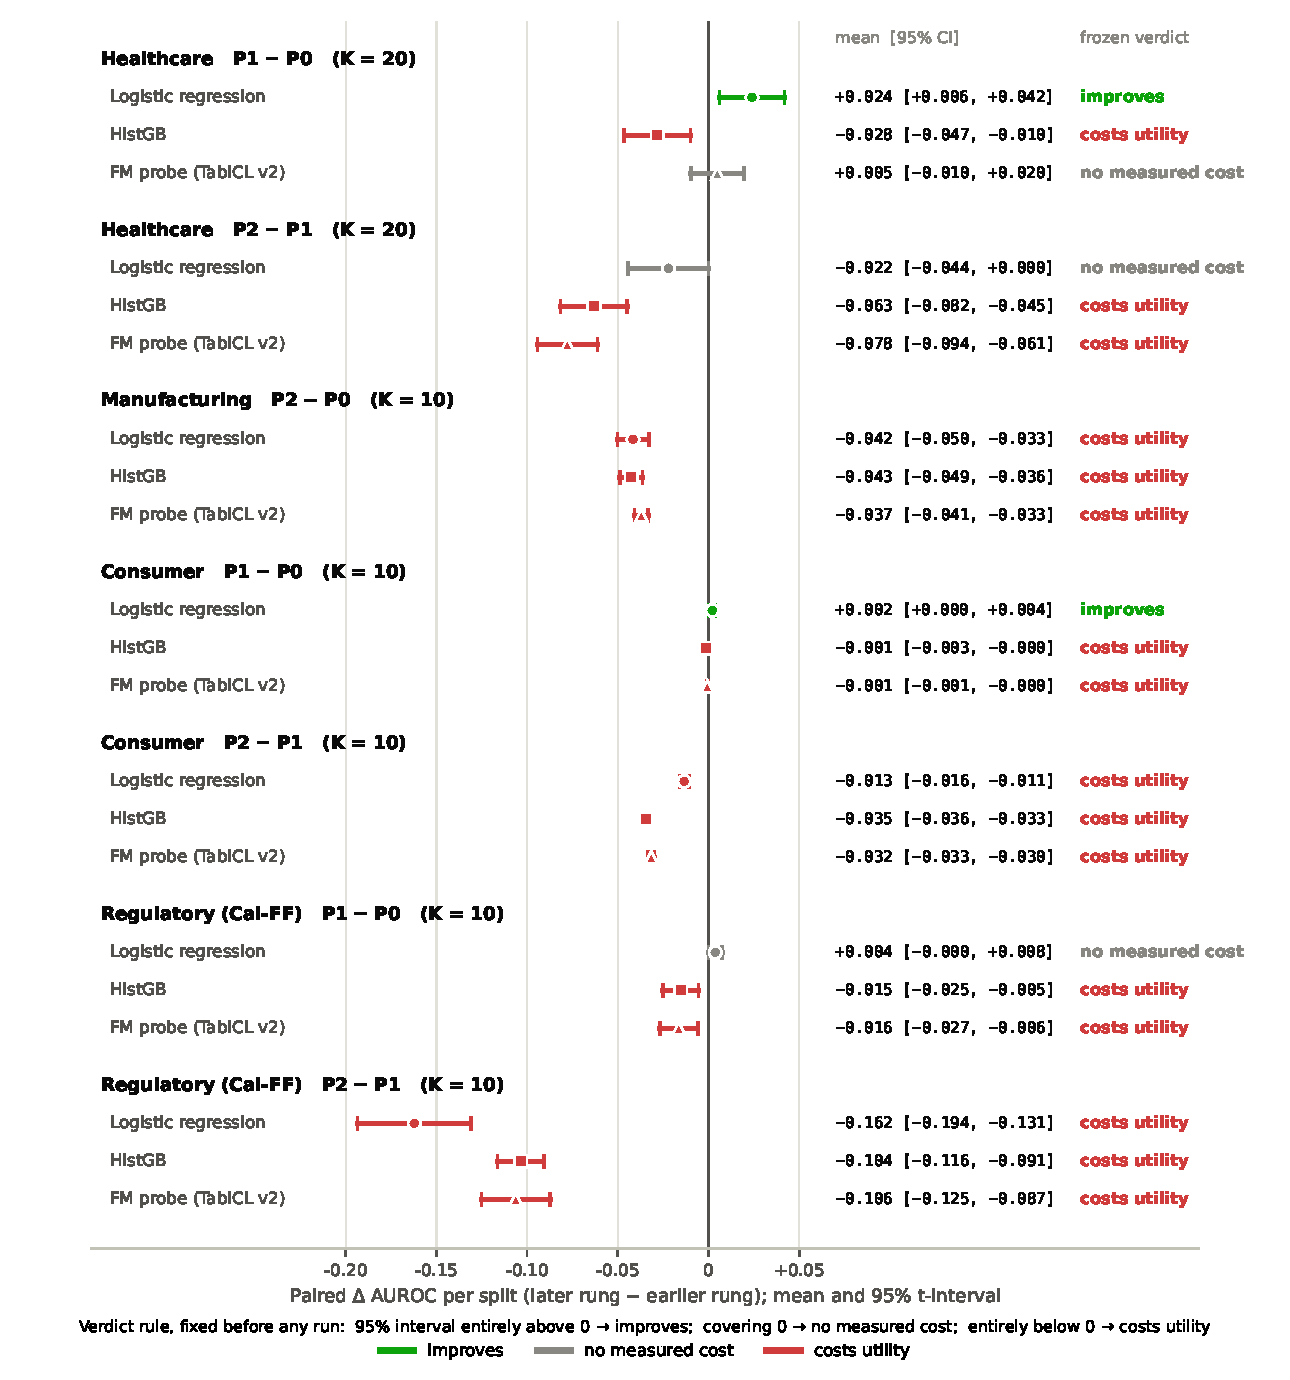
\includegraphics[width=0.92\textwidth]{figs/fig2_forest_7groups.pdf}
\caption{Paired per-split \dAUROC{} with 95\% $t$-intervals for every producer at every tested step, coloured by the frozen verdict. Manufacturing has no distinct \po{}.}
\label{fig:forest}
\end{figure}

Figure~\ref{fig:frontier} shows the frontier; Table~\ref{tab:means} gives the replicated means, Table~\ref{tab:deltas} and Figure~\ref{fig:forest} the paired deltas and verdicts.

\paragraph{The governed step is producer-dependent on the clinical task.} Moving from \pz{} to \po{} improved logistic regression ($+0.024$ [$+0.006$, $+0.042$]), produced no measured cost for the probe ($+0.005$ [$-0.010$, $+0.020$]) and cost HistGB ($-0.028$ [$-0.047$, $-0.010$]). The tree model had been using fields that the governed projection removes; the linear model had not benefited from them. This is one step, on one task, moving three producers in three directions.

\paragraph{The governed step is task-dependent for the same producer.} On the consumer task the same step is resolvable for all three producers but no larger than $0.002$ in magnitude at the reported precision---statistically detectable and practically negligible. On the regulatory task, where the step coarsens exact coordinates to county membership, it \emph{costs} the probe ($-0.016$ [$-0.027$, $-0.006$]) and HistGB ($-0.015$ [$-0.025$, $-0.005$]) and is no measured cost for logistic regression ($+0.004$ [$-0.000$, $+0.008$]). Coordinates carry signal for this target that county membership does not replace. The governed step is therefore neither free nor fixed-cost: it is measured per producer and per axis.

\paragraph{Aggressive minimization costs utility in eleven of twelve cells.} Eleven of the twelve \pt{} intervals exclude zero, from $-0.013$ (consumer, logistic) to $-0.162$ (regulatory, logistic). The twelfth, clinical logistic \pt$-$\po{} at $-0.022$ [$-0.044$, $+0.000$], has an upper bound a hair above zero ($+0.0001$ before rounding) and is therefore recorded as no measured cost; the rule was applied as written rather than adjusted after the fact.

\paragraph{The probe leads on replicated means, by modest and task-dependent margins.} At ten of the eleven task--level cells the probe has the highest mean AUROC (Table~\ref{tab:means}): clinical \po{} $0.655$ against $0.626$ (logistic) and $0.582$ (HistGB); manufacturing \pz{} $0.983$ against $0.975$ (HistGB) and $0.897$ (logistic); consumer \pz{} $0.938$ against $0.932$ (HistGB) and $0.893$ (logistic); regulatory \pz{} $0.819$ against $0.771$ (logistic) and $0.760$ (HistGB). The margins over the better baseline are $0.029$, $0.008$, $0.006$ and $0.048$. The exception is clinical \pt{}, where logistic regression ($0.604$) is ahead of the probe ($0.577$): once the aggregates alone remain, the probe loses more than the linear model does. Simple baselines remain close enough that measuring stays mandatory; this is not a general superiority result.

\subsection{A correction from replication}

The first, single-split run of the clinical task had placed logistic regression ahead of the probe at \po{} ($0.687$ against $0.623$) and this appeared in the falsification report as a finding. Across 20 splits the ordering reverses ($0.626$ against $0.655$). The single split was an upper-tail draw for the linear model. We report the v1 number here because it was pre-registered and recorded, and because the mechanism of its correction---split replication under a fixed environment---is what the rest of the paper depends on. The same pattern recurs in Study~2.

\section{Study 2: Evidence acquisition by reveal}
\label{sec:study2}

\subsection{Protocol}

The question is not what predicts the outcome but what to collect next. Fix a frozen predictor $f$ and a held-out case whose evidence is partitioned into classes. Withhold two classes, $c_1$ and $c_2$. For each withheld class $k$, estimate the predictor's \emph{sensitivity} to $k$ as the mean absolute change in $f$'s predicted probability over $M$ donor imputations of $k$'s fields (donors: the first $M$ training rows in a stable hash order; the other class remains withheld). Rank $c_1$ against $c_2$ by sensitivity. Then \emph{reveal} each class's true values in turn and measure the realized change $|f(\text{revealed}) - f(\text{withheld})|$. The case is scored correct if the top-ranked class produced the larger realized change. Cases whose two realized changes differ by less than a pre-set bar $\delta$ are excluded as indistinguishable and their count reported. A usefulness bar was fixed before any run: ranking accuracy $\ge 0.60$ with exact-binomial $p<0.05$ against $0.5$ on evaluable cases, and at least 30 evaluable cases; below it, usefulness is recorded as not established.

The protocol parameters were $M=8$, $\delta=0.005$, and a rotating assignment of class pairs by case index. The predictor is the same frozen probe as Study~1, fit once on each training split. On the clinical task the classes are conditions, medications, observations, encounters and immunizations (ten pairs), derived from column prefixes at the governed \po{} level. On the manufacturing task they are thermal, mechanical, wear and product type (six pairs); on the consumer task administrative, informational, product, engagement rates, calendar and---at \pz{} only---context codes (fifteen or ten pairs). Every class map was fixed from column names before its run.

\subsection{Results on the clinical task}

\begin{figure}[t]
\centering
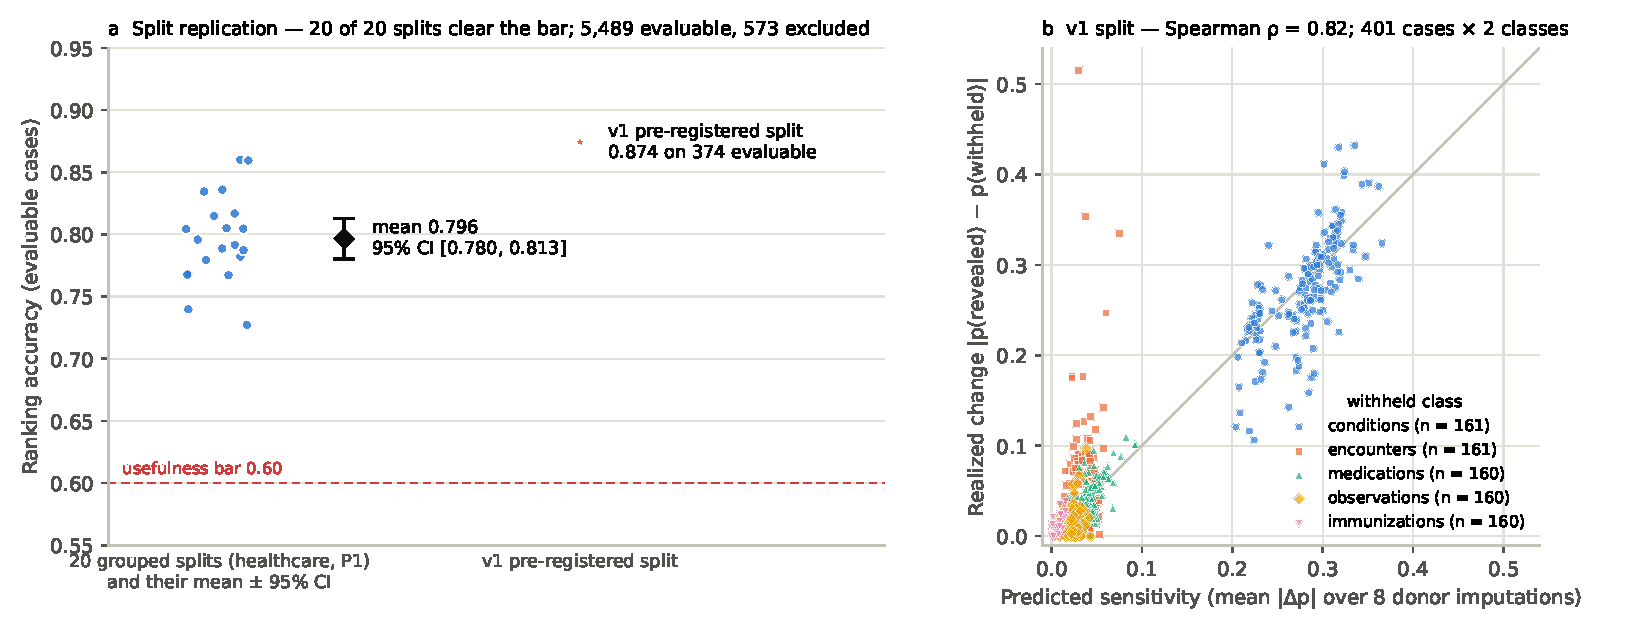
\includegraphics[width=\textwidth]{figs/fig3_acquisition.pdf}
\caption{(a) Ranking accuracy on 20 grouped clinical splits with mean and 95\% $t$-interval, beside the single pre-registered v1 split. (b) Predicted sensitivity against realized inference change for every withheld class-case on the v1 split.}
\label{fig:acq}
\end{figure}

\begin{table}[t]
\centering\small
\caption{Reveal-validated ranking across tasks. Exclusion is the share of held-out cases whose two realized changes were within $\delta=0.005$. Intervals are 95\% $t$-intervals over splits where $K>1$.}
\label{tab:acq}
\setlength{\tabcolsep}{4pt}\footnotesize
\begin{tabular}{@{}lccccccc@{}}
\toprule
Task, level & Classes / pairs & Cases & Evaluable & Excluded & Ranking accuracy & Spearman $\rho$ & Bar \\
\midrule
Healthcare, P1 (20 splits) & 5 / 10 & 6,062 & 5,489 & 573 (9\%) & 0.797 [0.780, 0.813] & 0.719 [0.698, 0.739] & 20/20 \\
Healthcare, P1 (v1 split) & 5 / 10 & 401 & 374 & 27 (7\%) & 0.874 & 0.823 & yes \\
Manufacturing, P0 & 4 / 6 & 2,996 & 1,608 & 1,388 (46\%) & 0.821 & 0.800 & yes \\
Consumer, P0 & 6 / 15 & 3,703 & 3,279 & 424 (11\%) & 0.915 & 0.900 & yes \\
Consumer, P1 & 5 / 10 & 3,703 & 3,231 & 472 (13\%) & 0.900 & 0.889 & yes \\
\bottomrule

\end{tabular}
\end{table}

The single pre-registered split gave 401 cases, 374 evaluable, ranking accuracy $0.874$ ($327/374$; exact binomial $p\approx 0$) and Spearman $\rho=0.82$ between predicted sensitivity and realized change across all withheld class-cases (Figure~\ref{fig:acq}b). Replicated over 20 grouped splits constructed by the same rule as Study~1, mean ranking accuracy was $0.797$ [$0.780$, $0.813$] (SD $0.035$; per-split range $0.727$--$0.860$), Spearman $0.719$ [$0.698$, $0.739$], with 5{,}489 evaluable cases and 573 excluded; all 20 splits cleared the usefulness bar (Figure~\ref{fig:acq}a, Table~\ref{tab:acq}). The v1 split was an upper-tail draw; the replicated interval controls the narrative, and $0.874$ is labelled as one split wherever it appears.

\paragraph{Where ranking is hard.} On the v1 split every pair involving conditions was ranked perfectly (161 of 161); the weakest pairs set encounters against observations ($0.59$ on 37 evaluable) and against medications ($0.60$ on 35). Predicted sensitivity tracks realized change for conditions ($0.279$ against $0.271$) and medications ($0.040$ against $0.037$), over-predicts observations ($0.024$ against $0.013$) and under-predicts encounters ($0.034$ against $0.052$)---the two classes behind most incorrect rows (Figure~\ref{fig:cal}b). Accuracy rises with the realized gap between the two withheld classes: $0.69$ for gaps in $[0.01, 0.02)$, $0.79$ in $[0.02, 0.05)$, $0.89$ in $[0.05, 0.10)$, $0.98$ above $0.10$; the smallest bin ($[0.005, 0.01)$, $n=22$) sits at $0.77$, so the curve is not strictly monotone at the low end (Figure~\ref{fig:cal}a). The protocol is hard exactly where the two classes barely differ, which the indistinguishability bar already partly removes.

\begin{figure}[t]
\centering
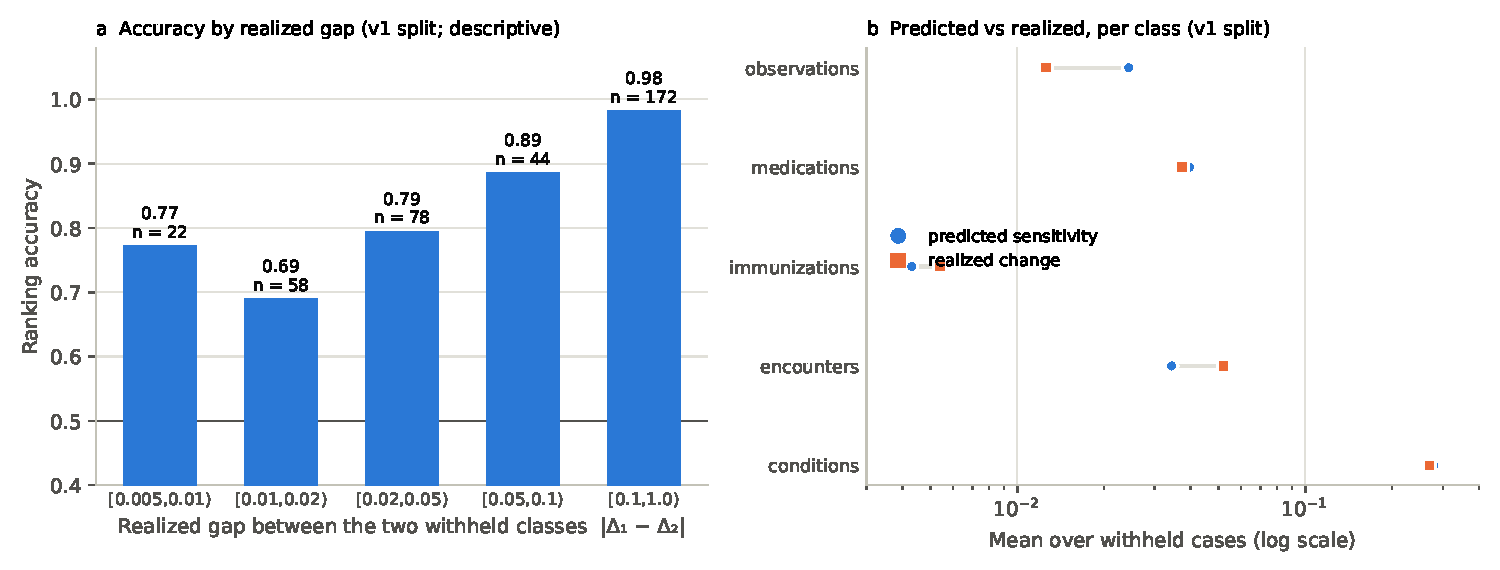
\includegraphics[width=\textwidth]{figs/fig6_calibration.pdf}
\caption{Descriptive re-aggregation of the frozen v1 rows. (a) Ranking accuracy by the realized gap between the two withheld classes. (b) Mean predicted sensitivity against mean realized change, per class.}
\label{fig:cal}
\end{figure}

\subsection{Protocol-parameter sensitivity}

\begin{table}[t]
\centering\small
\caption{One-factor-at-a-time sensitivity on the v1 split. The v1 protocol ($M=8$, $\delta=0.005$, v1 donor order, offset~0) remains the reported protocol; this is a robustness table, not tuning.}
\label{tab:sens}
\begin{tabular}{@{}llccc@{}}
\toprule
Factor & Setting & Evaluable & Ranking accuracy & Spearman $\rho$ \\
\midrule
donor imputations $M$ & 8 & 374 & 0.874 & 0.823 \\
donor imputations $M$ & 4 & 374 & 0.789 & 0.712 \\
donor imputations $M$ & 16 & 374 & 0.906 & 0.847 \\
\midrule
donor identity & v1 order & 374 & 0.874 & 0.823 \\
donor identity & alt.\ 1 & 374 & 0.909 & 0.865 \\
donor identity & alt.\ 2 & 374 & 0.901 & 0.862 \\
donor identity & alt.\ 3 & 374 & 0.890 & 0.850 \\
\midrule
indistinguishability bar & 0.002 & 390 & 0.862 & -- \\
indistinguishability bar & 0.005 & 374 & 0.874 & -- \\
indistinguishability bar & 0.01 & 352 & 0.881 & -- \\
indistinguishability bar & 0.02 & 294 & 0.918 & -- \\
\midrule
pair-rotation offset & 0 & 374 & 0.874 & 0.823 \\
pair-rotation offset & 5 & 364 & 0.860 & 0.816 \\
\bottomrule

\end{tabular}
\end{table}

\begin{figure}[t]
\centering
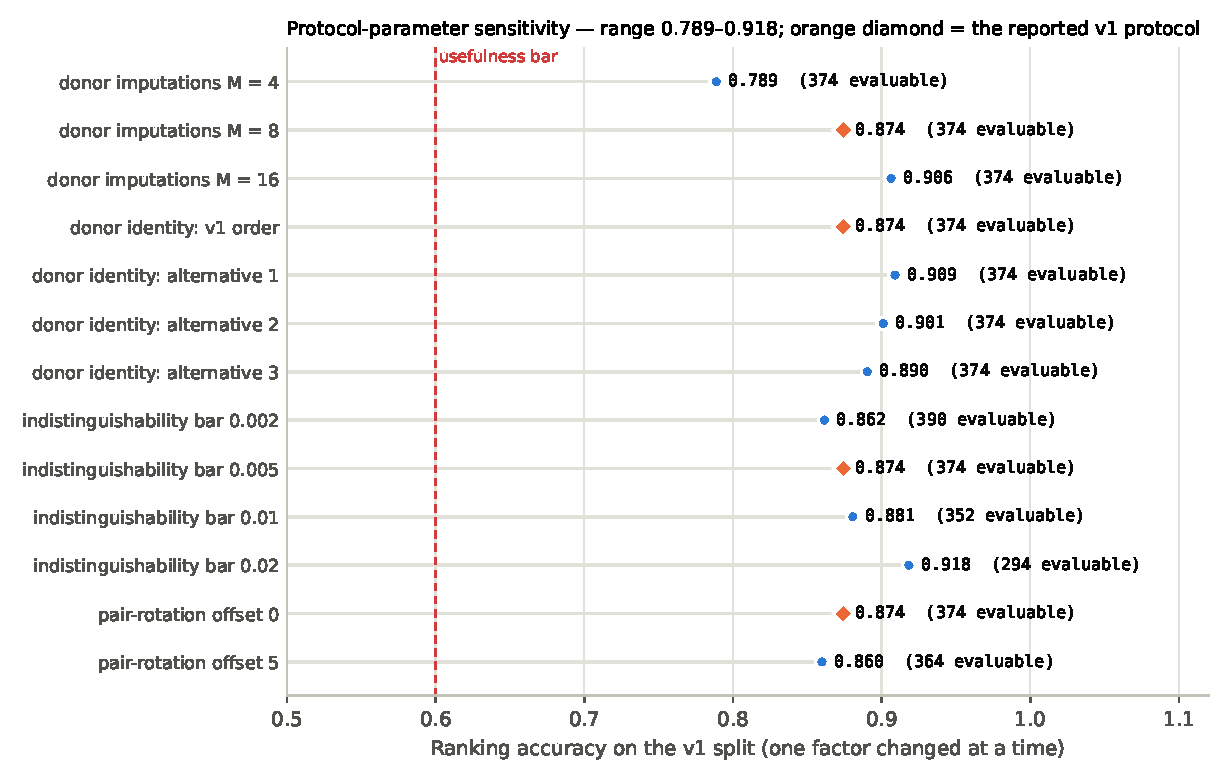
\includegraphics[width=0.9\textwidth]{figs/fig4_sensitivity.pdf}
\caption{Ranking accuracy on the v1 split as each protocol parameter is varied alone. Every cell clears the usefulness bar; the number moves most with the donor count $M$.}
\label{fig:sens}
\end{figure}

Table~\ref{tab:sens} and Figure~\ref{fig:sens} vary each hand-set parameter alone on the v1 split. Accuracy spans $0.789$--$0.918$ across all cells and clears the bar in every one. The donor count moves it most: $0.789$ at $M=4$, $0.874$ at $M=8$, $0.906$ at $M=16$---more imputations give a steadier sensitivity estimate. Donor identity matters modestly (three alternative orders: $0.890$--$0.909$). The bar trades rows for accuracy as expected ($\delta=0.002$: $0.862$ on 390; $\delta=0.020$: $0.918$ on 294). A different pair-rotation offset gives $0.860$. The result is robust in direction; its magnitude depends on $M$ and $\delta$, both of which should accompany any headline number.

\subsection{Second and third tasks}

\begin{figure}[t]
\centering
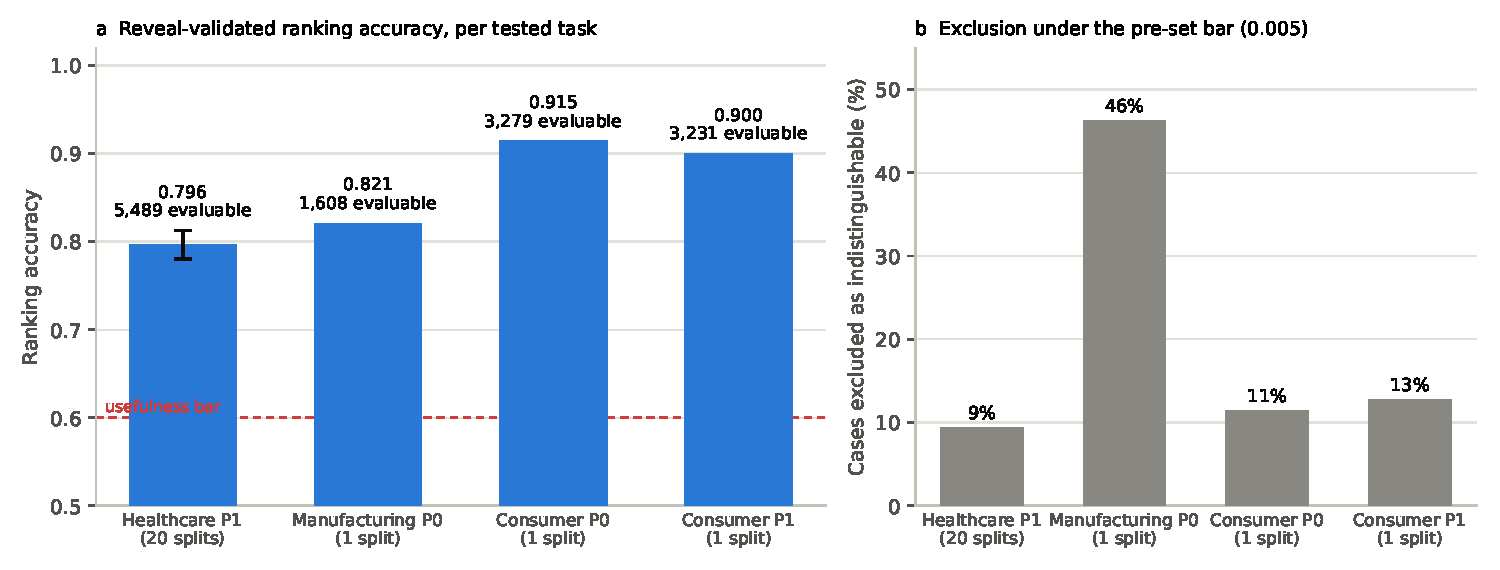
\includegraphics[width=\textwidth]{figs/fig5_tasks.pdf}
\caption{(a) Ranking accuracy per tested task (the clinical value is the 20-split mean with its interval). (b) Share of cases excluded as indistinguishable under the pre-set bar; the manufacturing task's low base rate leaves most cases with tiny realized changes.}
\label{fig:tasks}
\end{figure}

On the manufacturing task (AI4I, \pz), 2{,}996 held-out rows produced 1{,}608 evaluable cases---1{,}388 (46\%) were excluded, because a base rate of about 3.4\% (339 failures in 10{,}000 source rows) leaves most rows with realized changes below $\delta$. Ranking accuracy was $0.821$, Spearman $0.800$; the hardest pair was thermal against wear ($0.54$ on 56 evaluable, 443 excluded), the easiest product type against wear ($0.89$ on 490). On the consumer task, \pz{} gave $0.915$ on 3{,}279 evaluable (424 excluded, 11\%) and the governed \po{} $0.900$ on 3{,}231 (472 excluded, 13\%); the hardest pair at both levels was administrative against product ($0.64$ and $0.75$), two session-count classes whose realized changes are close. Every task clears the bar (Figure~\ref{fig:tasks}). The claim is ``for the tested tasks'', plural, and each number travels with its exclusion count.

\section{Replication in miniature on real de-identified records}
\label{sec:mimic}

The clinical task above is synthetic. To see whether the design behaves the same way on real records, we re-hosted it---producers, split rule, statistics and verdict rules unchanged---on the open MIMIC-IV Clinical Database Demo and MIMIC-IV-ED Demo (version 2.2; 100 de-identified patients; ODbL)~\citep{mimiciv,mimicdemo,mimiceddemo,physionet}. The plan was frozen before any model ran, after a test had confirmed that diagnosis codes cross the governed projection. Two structural differences were fixed in it: origins are patient event times rather than calendar dates, because MIMIC dates are shifted per patient, and diagnoses carry no onset or resolution dates. An origin is each hospital discharge the patient survived and each emergency-department discharge without admission; the label is an acute event within 365 days; of 310 candidate origins, 17 were excluded because the patient died in the window without an event and 55 because the window could extend past the patient's conservatively estimated end of observability. The cohort is 242 rows over 90 patients with a base rate of $0.587$; \pz{} has 111 fields, the governed \po{} 88 (23 fields removed by the governed projection), and \pt{} the same ten aggregate slots as the synthetic task. With $K=20$ grouped splits by patient the training sets hold 133--209 rows and the test sets 33--109, so the plan stated in advance that governed-step effects of Study~1's size would not be resolvable here and that a no-measured-cost verdict at that size is a statement about power.

\begin{table}[t]
\centering
\caption{Real-record miniature (MIMIC-IV demo, 242 rows, 90 patients, $K=20$): replicated AUROC by evidence level, mean (SD), and paired per-split $\dAUROC$ with 95\% $t$-intervals and the verdict under the pre-registered rule (I improves, N no measured cost, C costs utility).}
\label{tab:mimic}
\setlength{\tabcolsep}{4pt}\footnotesize
\begin{tabular}{lccclclc}
\toprule
Producer & $\pz$ & $\po$ & $\pt$ & $\po-\pz$ & & $\pt-\po$ & \\
\midrule
Logistic & 0.589 (0.092) & 0.612 (0.103) & 0.719 (0.067) & $+0.023$ [$-0.011$, $+0.056$] & N & $+0.108$ [$+0.051$, $+0.165$] & I \\
HistGB & 0.678 (0.074) & 0.645 (0.084) & 0.669 (0.069) & $-0.033$ [$-0.046$, $-0.020$] & C & $+0.024$ [$-0.011$, $+0.059$] & N \\
FM probe & 0.717 (0.062) & 0.703 (0.068) & 0.718 (0.061) & $-0.014$ [$-0.031$, $+0.003$] & N & $+0.015$ [$-0.010$, $+0.040$] & N \\
\bottomrule

\end{tabular}
\end{table}

Table~\ref{tab:mimic} gives the result. The governed step is again producer-dependent: it cost HistGB ($-0.033$ [$-0.046$, $-0.020$]), a resolved cell, and was no measured cost for logistic regression ($+0.023$ [$-0.011$, $+0.056$]) and for the probe ($-0.014$ [$-0.031$, $+0.003$]), with half-widths of $0.033$ and $0.017$. The aggressive step did not behave as it did on the synthetic task: it improved logistic regression by $+0.108$ [$+0.051$, $+0.165$] and was no measured cost for the other two producers. With 133--209 training rows and 88 fields, 60 of them sparse code indicators, the linear model is better served by ten aggregates; we report this as the observed frontier on this cohort, not as a mechanism. On this cohort the probe's replicated \po{} mean, $0.703$ (SD $0.068$), sits above HistGB's $0.645$ and logistic regression's $0.612$.

Acquisition by reveal transferred. At \po{}, over the same twenty splits, mean ranking accuracy was $0.828$ [$0.802$, $0.854$] (per-split range $0.690$--$0.912$) and Spearman $0.690$ [$0.653$, $0.726$], on 1{,}302 evaluable pair-cases with 95 (6.8\%) excluded as indistinguishable; the five classes were conditions, medications, observations, encounters and procedures. Nineteen of twenty splits cleared the usefulness bar; the twentieth had 27 evaluable cases against the pre-set minimum of 30 (its accuracy was $0.889$). The synthetic-task interval, $0.797$ [$0.780$, $0.813$], lies below this one.

Of the plan's five pre-registered hypotheses, two were met, two were not, and one was descriptive; the plan and both result files are released with the code so that a reader can score them. What the miniature supports is narrow and stated as such: the harness, the governed projection and both protocols execute on real de-identified records and return the same kinds of answer with wider intervals, and the one finding that changed direction---the aggressive step on the linear model---is also the one most exposed to the cohort size. It supports no claim about the hospital, its patients, or readmission in general, and ``real records'' here means an open 100-patient demonstration subset, not the credentialed database.

\section{Discussion}
\label{sec:discussion}

\paragraph{One axis, two directions.} Study~1 removes evidence and asks what utility survives; Study~2 withholds evidence and asks which class the predictor would most want back. The same frozen probe, environment and clinical splits serve both. Read together, they say that the evidence a model needs is neither a fixed quantity nor a fixed set: a linear model on the clinical task gained from the governed projection, the tree model lost, the probe was indifferent; and when asked which withheld class mattered, the probe was reliably right about conditions and unreliable about two low-signal classes whose effects were small and close.

\paragraph{The frontier is a curve, not a constant.} Across fifteen producer--step cells on the field-removal axis and six on the location-precision axis (21 in all: 16 costs, 3 no measured cost, 2 improvements), the governed step yielded every verdict the rule allows and the aggressive step yielded a cost in every cell but one at the boundary. A single ``price of privacy'' would have been wrong in both directions on the clinical task alone, and the real-record miniature (Section~\ref{sec:mimic}) moved the point further: the aggressive step that cost every producer on the synthetic task improved the linear model on 242 real rows. The practical reading is that minimization should be characterised empirically for the model and task at hand, with intervals, before any assurance is made about its cost or its harmlessness.

\paragraph{Corrections as method.} Both studies' first results were revised by replication over splits: a model ranking reversed in Study~1, and a headline accuracy fell by nearly eight points ($0.874$ to $0.797$) and acquired an interval in Study~2. Neither correction required a new hypothesis or a change of environment; it required more splits under the same pre-registered rule. We report the original numbers with their status rather than replacing them, because a reader who sees only the corrected figure cannot judge how much the design was doing.

\paragraph{Exclusion is part of the result.} The indistinguishability bar makes the acquisition score honest about cases where there was nothing to rank, and it also makes the score depend on the task's base rate: 9\% excluded on the clinical task, 46\% on manufacturing. Comparing accuracy across tasks without the exclusion count would compare different populations of cases.

\section{Limitations and claims ceiling}
\label{sec:limits}

The following are not supported by this evidence and are not claimed. Minimization is not shown to be free or to have a fixed cost; the governed projections carry no formal privacy, legal or identifiability guarantee; the probe is not shown to be generally superior to simple models; and nothing generalises beyond the four tasks, three producers, and the specific ladders tested. The regulatory label is not the source paper's matcher, and no facility-level finding is claimed. In Study~2, ranking accuracy is acquisition value under the frozen predictive capability---what would most alter \emph{this model's} output---not causal importance of any variable and not a data-collection policy; the per-class and per-gap analyses are descriptive re-aggregations of frozen rows; and the manufacturing and consumer results are single splits with class maps we defined. Re-execution of Study~1's three field-removal tasks on the originating machine in its current environment reproduced all 39 reported cells to four decimals, including the probe's; the regulatory task and Study~2 have not yet been re-executed. A companion replay harness that re-ran logistic regression and HistGB on two of the same source datasets (AI4I, Online Shoppers) under two other scikit-learn minor versions reproduced every logistic-regression output bit-for-bit but none of the HistGB outputs, with AUROC shifts of up to $0.004$, so HistGB cells should be read as environment-bound at the third decimal. The miniature of Section~\ref{sec:mimic} has test sets of 33--109 rows; its cohort is an ICU-weighted open demonstration subset whose base rate differs from the synthetic task's; its no-measured-cost verdicts have half-widths up to $0.035$ and are power statements; and its records, though real, are de-identified and openly licensed, with no patient-level finding reported. The synthetic clinical records carry no patient data and no claim about real records.

\section{Reproducibility}

Source data: Synthea synthetic records (no patient data); AI4I 2020 and UCI Online Shoppers (CC BY 4.0); Cal-FF (CC0-1.0); MIMIC-IV Clinical Database Demo and MIMIC-IV-ED Demo, version 2.2 (PhysioNet, ODbL 1.0; the twelve files read are verified against the published checksums). Every projection and the probe checkpoint are content-addressed; each result file records the projection hashes, split identities, seeds, protocol parameters, class maps, probe identity and harness code digest that produced it. Tables~\ref{tab:means}--\ref{tab:sens} and~\ref{tab:mimic} are generated from those files by script. The pre-registration plans, their recorded amendments, the claims boundary, and the result files will be released with the code.

\small
\bibliographystyle{unsrtnat}
\begin{thebibliography}{99}
\bibitem[European Parliament and Council(2016)]{gdpr} Regulation (EU) 2016/679 (General Data Protection Regulation), Article 5(1)(c): data minimisation. \emph{Official Journal of the European Union}, L119, 2016.
\bibitem[Howard(1966)]{howard1966} R.~A. Howard. Information value theory. \emph{IEEE Transactions on Systems Science and Cybernetics}, 2(1):22--26, 1966.
\bibitem[Saar-Tsechansky et~al.(2009)]{saartsechansky2009} M.~Saar-Tsechansky, P.~Melville, and F.~Provost. Active feature-value acquisition. \emph{Management Science}, 55(4):664--684, 2009.
\bibitem[Shim et~al.(2018)]{shim2018} H.~Shim, S.~J. Hwang, and E.~Yang. Joint active feature acquisition and classification with variable-size set encoding. In \emph{Advances in Neural Information Processing Systems 31}, 2018.
\bibitem[Pedregosa et~al.(2011)]{sklearn} F.~Pedregosa et~al. Scikit-learn: Machine learning in Python. \emph{Journal of Machine Learning Research}, 12:2825--2830, 2011.
\bibitem[Qu et~al.(2025)]{tabicl} J.~Qu, D.~Holzm\"{u}ller, G.~Varoquaux, and M.~Le~Morvan. TabICL: A tabular foundation model for in-context learning on large data. In \emph{Proceedings of the 42nd International Conference on Machine Learning}, 2025.
\bibitem[Walonoski et~al.(2018)]{synthea} J.~Walonoski et~al. Synthea: An approach, method, and software mechanism for generating synthetic patients and the synthetic electronic health care record. \emph{Journal of the American Medical Informatics Association}, 25(3):230--238, 2018.
\bibitem[Matzka(2020)]{ai4i} S.~Matzka. Explainable artificial intelligence for predictive maintenance applications. In \emph{Third International Conference on Artificial Intelligence for Industries (AI4I)}, pages 69--74, 2020.
\bibitem[Sakar et~al.(2019)]{shoppers} C.~O. Sakar, S.~O. Polat, M.~Katircioglu, and Y.~Kastro. Real-time prediction of online shoppers' purchasing intention using multilayer perceptron and LSTM recurrent neural networks. \emph{Neural Computing and Applications}, 31:6893--6908, 2019.
\bibitem[Johnson et~al.(2023)]{mimiciv} A.~E.~W. Johnson, L.~Bulgarelli, L.~Shen, et~al. MIMIC-IV, a freely accessible electronic health record dataset. \emph{Scientific Data}, 10:1, 2023.
\bibitem[Johnson et~al.(2023)]{mimicdemo} A.~Johnson, L.~Bulgarelli, T.~Pollard, S.~Horng, L.~A. Celi, and R.~Mark. MIMIC-IV Clinical Database Demo (version 2.2). PhysioNet, 2023. doi:10.13026/dp1f-ex47.
\bibitem[Johnson et~al.(2023)]{mimiceddemo} A.~Johnson, L.~Bulgarelli, T.~Pollard, L.~A. Celi, S.~Horng, and R.~Mark. MIMIC-IV-ED Demo (version 2.2). PhysioNet, 2023. doi:10.13026/jzz5-vs76.
\bibitem[Goldberger et~al.(2000)]{physionet} A.~L. Goldberger, L.~A.~N. Amaral, L.~Glass, et~al. PhysioBank, PhysioToolkit, and PhysioNet: Components of a new research resource for complex physiologic signals. \emph{Circulation}, 101(23):e215--e220, 2000.
\bibitem[Stanford RegLab(2025)]{calff} Stanford Regulation, Evaluation, and Governance Lab. Cal-FF: A comprehensive dataset of factory farms in California. \emph{Scientific Data}, 2025. \href{https://doi.org/10.1038/s41597-025-06082-6}{doi:10.1038/s41597-025-06082-6}.
\end{thebibliography}

\end{document}
